\documentclass{article}

% NeurIPS 2026 style, camera-ready: `final` names the author and drops the line numbers.
\usepackage[final]{neurips_2026}

% The workshop asks for this footnote: "Submitted to/Accepted at/Published in the AI for Science
% workshop (NeurIPS 2026)."
\makeatletter
\renewcommand{\@noticestring}{Accepted at the AI for Science workshop (NeurIPS 2026).}
\makeatother

\usepackage[T1]{fontenc}
\usepackage[utf8]{inputenc}
\usepackage{array}
\usepackage{booktabs}
\usepackage{amsmath}
\usepackage{amssymb}
\usepackage{xcolor}
% One reference carries a 150-character URL, a single token wider than the text block.
% url breaks it on any character rather than overflowing the margin.
\usepackage{url}
\def\UrlBreaks{\do\/\do\-\do\.\do\_\do\?\do\&\do\=\do\+}
\usepackage{hyperref}
\usepackage{natbib}
\usepackage{caption}
\usepackage{graphicx}
% Appendix floats sit where they are written: a heading must not be parted from its table or figure.
\usepackage{float}
\usepackage{longtable}
\usepackage{needspace}

\hypersetup{colorlinks=true, linkcolor=black, citecolor=black, urlcolor=blue}
\captionsetup{font=small}

% Long unbreakable tokens (JSON pointers, command names) in narrow p-columns overflowed
% six paragraphs. A final-pass stretch is the standard remedy and changes nothing else.
\setlength{\emergencystretch}{3em}

\newcommand{\TODO}[1]{\textcolor{red}{\textbf{[TODO:}~#1\textbf{]}}}
\newcommand{\FILLIN}[1]{\textcolor{red}{\textbf{[FILL-IN:}~#1\textbf{]}}}
\newcommand{\REVIEW}[1]{\textcolor{orange}{\textbf{[REVIEW:}~#1\textbf{]}}}
\newcommand{\code}[1]{\texttt{#1}}

% Float separation is one length for above and below, so a table set tight against the paragraph
% under it needs both widened. The gap between a caption and the table it heads comes from the
% style, which sets it for a caption placed above the tabular as NeurIPS requires.
\setlength{\intextsep}{14pt plus 3pt minus 2pt}
\setlength{\textfloatsep}{18pt plus 3pt minus 2pt}

% The commands, named once so a rename is one edit.
\newcommand{\sys}{Reproducible Science}
\newcommand{\Sys}{Reproducible Science}
\newcommand{\tPlan}{\code{prereg}}
\newcommand{\tRun}{\code{results}}
\newcommand{\tCite}{\code{citations}}
\newcommand{\tVerify}{\code{repro}}
\newcommand{\tVerifyCmd}{\code{repro verify}}

\title{Reproducible Science: Machine-Checkable Claims\\from Preregistration to Publication}
\author{Elliot Tower\\\texttt{elliot@elliottower.ai}}
\date{}

\begin{document}
\maketitle

\begin{abstract}
Every claim in a paper comes from somewhere. AI tooling allows us to quickly generate hypotheses,
run analyses, and draft manuscripts, but we identify verification and provenance as open issues:
(1)~verifying that the finished paper agrees with the artifacts behind it typically requires
manual or agentic verification, which is expensive and difficult to audit; (2)~verification
usually does not include a denominator for the number of sources or artifacts checked;
(3)~verification snapshots quickly become stale, and are not guaranteed to find every issue or
reproduce the same issues on subsequent runs; (4)~more experiments means more researcher degrees
of freedom and post-hoc analysis, even if unintentional, or done by an agent; and
(5)~verification is typically done post-hoc, and does not cover all steps of the research
lifecycle.

We present Reproducible Science\footnote{Package: \url{https://github.com/elliottower/reproducible-science}}, a declarative, continuous, machine-checkable provenance layer
for research claims, throughout the whole research lifecycle. \tPlan{} freezes a plan before the
run, \tRun{} seals its inputs, records its outputs and binds numbers in the manuscript to the run
that produced them, \tCite{} pins exact quotations inside cited sources, and \tVerify{} checks
every declaration against the artifact it names. Our Claude Code plugin records provenance at the
time of experimentation and reports drift on every edit through hooks. Applying this contract to
this paper\footnote{Paper code and artifacts: \url{https://github.com/elliottower/reproducible-science-paper}} surfaced two errors, one of which had already gone stale twice. As agents take over more
of the research lifecycle, the artifacts they leave behind are worth only as much as we can verify
the claims inside them.
\end{abstract}

% AI tooling allows us to quickly generate hypotheses,
% run analyses, and draft manuscripts, but verification and provenance remain open issues.
% Every claim in a paper comes from somewhere. We present Reproducible Science, a continuous,
% machine-checkable provenance layer for research claims. Command-line tools freeze a plan before
% the run, seal its inputs and record its outputs, bind every number in the manuscript to the run
% that produced it, and locate every quotation inside the source it cites. Our Claude Code plugin
% records provenance at the time of experimentation and reports drift on every edit through hooks.
% We are motivated by the following problems. 1.)~Verifying that the finished paper agrees with the artifacts behind it typically requires
% manual or agentic verification---which produces yet another difficult-to-audit verdict;
% 2.)~Verification usually does not include a denominator for the number of sources or artifacts
% checked; 3.)~Verification snapshots quickly become stale, and are not guaranteed to find every
% issue or reproduce the same issues on subsequent runs. 4.)~More experiments means more researcher
% degrees of freedom and post-hoc analysis---even if unintentional, or done by an agent.
% 5.)~Verification is typically done post-hoc, after results and context windows may have
% disappeared.
% 1.)~verifying that the finished paper agrees with the artifacts behind it typically requires
% manual or agentic verification---which produces yet another difficult-to-audit verdict;
% 2.)~verification usually does not include a denominator for the number of sources or artifacts
% checked; 3.)~verification snapshots quickly become stale, and are not guaranteed to find every
% issue or reproduce the same issues on subsequent runs. 4.)~more experiments means more researcher
% degrees of freedom and post-hoc analysis---even if unintentional, or done by an agent.
% 5.)~verification is typically done post-hoc, after results and context windows may have
% disappeared.
% This software solves the following problems: 1.)~verifying that the finished paper agrees with the artifacts behind it typically requires
% manual or agentic verification---which produces yet another difficult-to-audit verdict;
% 2.)~verification usually does not include a denominator for the number of sources or artifacts
% checked; 3.)~verification snapshots quickly become stale, and are not guaranteed to find every
% issue or reproduce the same issues on subsequent runs. 4.)~More experiments means more researcher
% degrees of freedom and post-hoc analysis---even if unintentional, or done by an agent.
% 5.)~Verification is typically done post-hoc, after results and context windows may have
% disappeared.
% Over an audit of 2{,}512 quotations against 125 content-addressed sources, 113 failed to resolve
% and none was a misquotation. Every failure came from extraction --- which a two-state report
% records as an accusation against the manuscript.
% \end{abstract}

\section{Introduction}
\label{sec:intro}

Surveys of research agents name verification as the step that has not kept pace
\citep{ding2026verificationgap}. Re-running the analysis is the usual answer, and it is
usually unavailable: across 863{,}878
attempted executions of valid notebooks, 24.11\% ran without errors and 4.03\% produced the
results the notebook recorded \citep{pimentel2019notebooks}. The deeper problem is that
re-running checks the wrong object. A notebook that re-executes perfectly can still sit beside a
manuscript printing a value no output contains, because execution establishes that the code runs
and says nothing about what the paper claims the code produced. Reproducibility and verification
are different properties. A project can preserve its code, its data and its logs and still
print a value no output contains, quote a passage that was never read out of its source, or call an analysis
confirmatory after its plan changed.

We call what accumulates \textbf{verification debt}. Like debt in software, it is cheapest to
detect when it is introduced and expensive to reconstruct afterwards. At the moment a value
changes, the run that produced the old one is still on disk, the source still resolves, and the
edit carries an author and a commit. Later the run has been overwritten, the source was fetched
once without its address recorded, and which document a citation referred to is no longer
recoverable from the citation. In 14 of 34 documented cases of retraction, correction, or
misconduct, the toolkit's checks would flag a stated problem, including both Surgisphere
COVID-19 studies (Appendix~\ref{sec:failure-cases}).

\begin{table}[h]
\centering
\small
\caption{Three boundaries of a research project, the failure each admits when nothing checks it,
and the comparison the toolkit performs. All three are decided the same way, by a digest of a file
and a comparison at a location the author declares in it, so one checking engine serves them.}
\label{tab:boundaries}
\begin{tabular}{@{}>{\raggedright\arraybackslash}p{0.23\textwidth}>{\raggedright\arraybackslash}p{0.38\textwidth}>{\raggedright\arraybackslash}p{0.29\textwidth}@{}}
\toprule
\textbf{Boundary} & \textbf{What goes wrong when it is unchecked} & \textbf{What the toolkit compares} \\
\midrule
plan to run & a hypothesis or an analysis is rewritten after the outcome is visible & a run record against a plan pinned by digest \\
run to manuscript & a printed value drifts from the output it was read from & a declared address in a sealed result file \\
source to manuscript & a quotation or an identifier does not occur in the artifact cited for it & a passage against a content-addressed source \\
\bottomrule
\end{tabular}
\end{table}

Most of what a reader would want checked is not mechanically checkable: whether a design answers
the question, whether a conclusion follows. A narrow part is. A number printed in a manuscript
either matches the results file it came from or does not, and a quoted sentence either occurs in
the cited source or does not. That part can be settled without a human and without a model, at a
cost small enough to run on every commit rather than once before submission.

\begin{figure}[h]
\centering
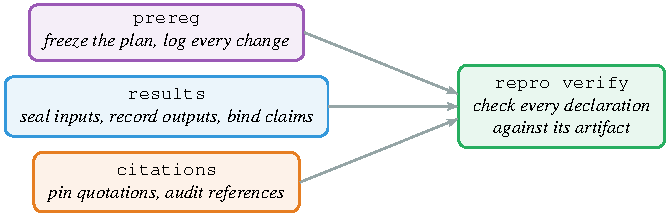
\includegraphics[width=0.56\textwidth]{figures/fig_commands.pdf}
\caption{The toolkit's four commands. \tPlan{}, \tRun{} and \tCite{} each write declarations while the work
is done, and \tVerifyCmd{} reads them and checks each against the artifact it names.}
\label{fig:commands}
\end{figure}

\paragraph{Nothing failed because nothing ran.} In the toolkit's own code, a missing extractor, the program that pulls text out of a
PDF, returned the empty string, the check recorded an unreadable document, and the run summary read
\emph{nothing failed}. A check that read no text and a check that read the text and found it
correct produced the same line. A separate incident is worse: a script collected the digests cited
by every registration under one directory and verified each against a file; the directory was
renamed, the glob matched nothing, the script exited zero, and continuous integration, a pre-push
hook and a make target were all green in that state. A report that returns success is not evidence
that anything was examined, and an outcome vocabulary with no term for non-execution cannot say so.

\paragraph{Position.} Three claims follow, each against a live alternative. \emph{Prospective decisions
require prospective records}: a frozen plan cannot establish that an author was honest, but it
makes subsequent rewriting detectable and separates confirmatory work from exploratory work.
\emph{Evidence requires declared addresses}: a reported \code{0.42} should name the pointer or
selector it came from, because searching afterwards for a numerically similar value is not
provenance and does not scale. The alternative is to recover the address afterwards, and a contemporaneous system does:
Paperclip binds the same unit, a claim to a location in a source, and verifies it with a
language-model subagent against line ranges into its own re-parse \citep{gxl2026paperclip}. A
verdict from a model is not recomputable from the artifact, and an address into a re-parse moves
when the parser improves. We make the opposite choice on both: the comparison is deterministic,
and an address points into pinned bytes. \emph{Verification requires an explicit non-execution state}: a
checker that cannot distinguish matched, disagreed, absent and could-not-run has no way to report
that a green build examined nothing. Our own infrastructure violated the non-execution
requirement twice.

\paragraph{Contributions.} (1)~\textbf{Lifecycle verification}: a model spanning the
plan-to-run, run-to-manuscript and source-to-manuscript boundaries of Table~\ref{tab:boundaries},
designed to run while a project changes. (2)~\textbf{Evidence assertions}: typed assertions binding
manuscript values and quotations to declared locations in content-addressed artifacts, with four
implemented variants over a shared engine and report. (3)~\textbf{Staged outcomes}: a deterministic
model separating execution, extraction and comparison, with a project's pass-or-fail policy applied
to the resulting facts afterwards. We instantiate all three in a deployed toolkit (Figure~\ref{fig:commands}) and
evaluate them through conformance tests, fault injection, a content-addressed quotation audit,
defects met in ordinary use, and an audit of a project developed using this toolkit.


\section{Model and Contract}
\label{sec:construction}

Section~\ref{sec:intro}'s two incidents fail differently --- one check never ran, the other ran
and read no text --- and both reported what a passing check reports. The three boundaries of
Table~\ref{tab:boundaries} share one architecture: declare an address, pin the
artifact it points into, compare deterministically, and report each stage separately. Two of the three are decided by an \emph{evidence assertion}, which
binds a manuscript claim to an artifact, a locator within it, and the value or passage expected
there. A project lists its assertions in one file, the manifest. The plan-to-run boundary is decided by reading a run record beside a pinned plan, so no
evidence assertion is defined for it. Four variants are implemented across the other two
boundaries. They differ in how evidence is located and compared, and share artifact pinning,
staged outcomes and one report. Appendix~\ref{sec:terms} provides the full definition of each term used here.

\begin{table}[h]
\centering
\small
\caption{The four implemented variants. A table cell is addressed by a selector over key columns,
because a row index addresses a different cell when the table is reordered. A correspondence names
no expected value: neither side is the reference, and a disagreement prints both readings.}
\label{tab:contract}
\begin{tabular}{@{}>{\raggedright\arraybackslash}p{0.15\textwidth}>{\raggedright\arraybackslash}p{0.26\textwidth}>{\raggedright\arraybackslash}p{0.21\textwidth}>{\raggedright\arraybackslash}p{0.27\textwidth}@{}}
\toprule
\textbf{Kind} & \textbf{Assertion} & \textbf{Located by} & \textbf{Compared how} \\
\midrule
metric & this artifact holds this value here & RFC 6901 JSON Pointer & decimal, at the precision the manuscript printed \\
table & this table holds this value in this cell & column plus a row selector & decimal, at the precision the manuscript printed \\
quote & this passage occurs in this artifact & page, optionally & verbatim after normalization that preserves which words appear \\
correspondence & two artifacts hold the same value & a locator on each side, prose anchors or a pointer & decimal, at the precision the manuscript printed \\
\bottomrule
\end{tabular}
\end{table}

\paragraph{Three stages.} A check must execute, extract, and compare, and the three fail
independently. Table~\ref{tab:stages} gives the outcomes and the flattened view derived from them.
The rows differ in what a reader should do: revise the claim, fix the pointer or run the analysis
that produces the value, install a package, file a bug. A report that cannot distinguish them
directs none of those actions.

\begin{table}[h]
\centering
\small
\caption{The three stages and the flattened view derived from them, the single label a report
prints. A pointer to a key the results file lacks is reported \code{not\_found}: nothing is
asserted about whether the value differs. An extractor that is not installed yields
\code{unchecked}, and an extractor that raises yields \code{error} and never \code{unchecked}.}
\label{tab:stages}
\begin{tabular}{@{}>{\raggedright\arraybackslash}p{0.34\textwidth}lll>{\raggedright\arraybackslash}p{0.15\textwidth}@{}}
\toprule
\textbf{Situation} & \textbf{Execution} & \textbf{Extraction} & \textbf{Comparison} & \textbf{Flattened} \\
\midrule
value present & completed & extracted & match & \code{verified} \\
value differs in a readable artifact & completed & extracted & mismatch & \code{mismatch} \\
pointer does not resolve & completed & absent & --- & \code{not\_found} \\
extractor not installed & unavailable & not attempted & --- & \code{unchecked} \\
backend defect & failed & not attempted & --- & \code{error} \\
\bottomrule
\end{tabular}
\end{table}

\paragraph{Pins.} Artifacts are content-addressed, and pins are resolved before any evidence is
read, so a source that moved is known before decisions are computed against it. Decisions against
a broken or unpinned artifact still run and are reported, marked non-authoritative, because a
diagnostic is more useful than a blank.

\paragraph{Facts, then policy.} Verification returns facts. Whether they constitute a pass depends
on what the project is for: an unchecked citation is acceptable in a draft and disqualifying in a
submission, and both readings are correct about the same run. The engine therefore reports the
three stages and computes no verdict, and a profile maps outcomes to severities
(Table~\ref{tab:policy}, Appendix~\ref{sec:suite}). Re-grading under
a stricter profile re-reads the stored report and executes nothing, so a submission is judged on
the facts the draft was checked with rather than on a second run that may not reproduce them.

\section{Implementation and Workflow}
\label{sec:use}

The toolkit runs on ordinary files. It does not require an experiment to be conducted in a
particular language, notebook system, analysis framework or agent runtime, and it does not require
a manuscript to be authored inside its toolchain. The fifteen papers in the quotation audit of Section~\ref{sec:quote} were
written without this contract in mind, and none was modified to be auditable. A value is read
from JSON, delimited text, a workbook, Parquet, Stata, SPSS, R data, HDF5 or NetCDF, and a
quotation from a PDF, plain text, a workbook, a Word document or JATS XML.

A new or existing project adopts the toolkit with one command, \code{repro init}. A project declares as it goes. A plan is frozen before the run it governs, against a commit and a
content hash. Inputs are sealed before an analysis and outputs recorded after it. The script is
committed, its inputs are sealed and its outputs are recorded, so every result can be regenerated:
\code{repro reproduce} runs the declared command again and checks the manuscript's assertions
against the file it writes. Misconduct that alters a reported result now requires more than an edit to the
manuscript: the committed script must produce the altered value from the sealed inputs, and a
re-run by a reader reveals any inconsistency. For each sentence that prints a number, the manifest records the address the number came from,
written when the sentence is. Verification then reads the declarations and reports on each.

\begin{table}[h]
\centering
\small
\caption{The toolkit's four commands and the boundary each decides. The first three write declarations
and the fourth reads them, applying a policy to the result.}
\label{tab:commands}
\begin{tabular}{@{}>{\raggedright\arraybackslash}p{0.13\textwidth}>{\raggedright\arraybackslash}p{0.80\textwidth}@{}}
\toprule
\textbf{Command} & \textbf{What it establishes} \\
\midrule
\tPlan{} & that the plan which ran is the plan that was frozen, against a commit and a content hash \\
\tRun{} & that a reported number came from a recorded run over sealed inputs \\
\tCite{} & that a quoted passage occurs in the source cited for it \\
\tVerify{} & that every declared assertion holds against its pinned artifact, and which do not \\
\bottomrule
\end{tabular}
\end{table}

\paragraph{A worked example.} Appendix~\ref{sec:suite} states that the conformance suite holds 25
fixtures, and this paper's manifest binds that sentence with two assertions: a \code{quote}
assertion checking that the manuscript still prints it, and the \code{metric} assertion below,
checking that the pinned inventory of the suite holds the number at the declared pointer.
{\footnotesize
\begin{verbatim}
- kind: metric
  artifact: conformance     # pinned: sha256 b9840b9d...
  pointer: /fixtures
  reported: '25'

$ repro verify --policy strict
  ok    conformance-fixtures metric   /fixtures = 25
  72 verified
  policy strict: passed  (0 errors, 0 warnings)
\end{verbatim}}
\noindent With \code{reported: '19'}, the stale count of Section~\ref{sec:selfaudit}, the line is
marked \code{MISS}, the run exits 1, and the report reads \emph{manuscript prints 19,
conformance\_inventory.json holds 25}. The Claude Code plugin prompts for such
declarations while the artifacts are produced: after each edit it names any number or quotation in
a manuscript that nothing yet backs, and before an analysis runs it says when the governing plan is
unfrozen, never blocking the work it observes. A companion Claude Code mod shows the state of a project's
records in the session, one row per command, with a warning when a frozen plan was edited or a run
was recorded with nothing sealed (Appendix~\ref{sec:status}, Figure~\ref{fig:status}).

Preregistration is optional and per claim. A claim is marked confirmatory, exploratory, or not
applicable, and only the first requires a plan behind it. This matters for the honesty of the
report: a project that registers nothing is not failed for it, and a project that calls a claim
confirmatory is held to the plan it named.

Cost is what makes the check a commit-time one. Verifying this paper's 76 assertions over 25 artifacts takes 0.53 seconds; resolving its
63 quotations against 17 content-addressed sources takes 4.10 seconds
(Appendix~\ref{sec:timing}).

\section{Evaluation}
\label{sec:eval}

The conformance suite and the fault injections are in Appendix~\ref{sec:suite}: 25 fixtures,
each recording its expected outcome, reason and artifact validity as a triple so a case
cannot pass by reaching the right verdict for the wrong cause, and four injected faults each
distinguishing a class the flattened view would otherwise merge.

\subsection{Self-audit}
\label{sec:selfaudit}

This paper is an instance of what it describes. Each number its manifest binds carries two assertions: that the manuscript states
the sentence, and that a pinned artifact holds the value at a declared pointer. Thirty-eight claims are
bound this way, 76 assertions over twenty-five artifacts, and they pass under the \code{strict} policy
profile. The manifest and the artifacts it pins are in the repository, so the check is one a
reader runs rather than a result they take on trust. No claim here is confirmatory, so none requires a
registered plan.

Building the manifest surfaced two defects in this paper's own numbers. Four counts in
Table~\ref{tab:readers} had been computed correctly and written to no file, so nothing could
re-check them; derived into an artifact, all four match what the manuscript prints. The count of
conformance fixtures was recorded and stale: a stored figure gave nineteen where the suite holds
25, and the specification had earlier stated eighteen against a count of nineteen.

\subsection{Quotation audit}
\label{sec:quote}

Six extractors read the same 2{,}364 passages, quoted from fifteen published papers, out of the same pinned bytes and returned six
different answers, from 2{,}314 down to 1{,}716 (Table~\ref{tab:readers}). A verification snapshot therefore records the
reader as much as the corpus, and a rerun under a different toolchain is not guaranteed to find
the same issues. Under poppler's layout mode 113 quotations fail to resolve and every failure
traces to extraction (Appendix~\ref{sec:suite}), so a checker with only pass and fail would have
accused the manuscripts 113 times with no misquotation present.

\subsection{Recall against CORE-Bench}

The corpora above carry no ground truth: nobody has labelled which of a paper's numbers its
artifact really holds, so a located value is evidence of an occurrence. CORE-Bench supplies the missing half, and a bound: a value no reader finds in an artifact is a
value no assertion can point to. Each capsule, CORE-Bench's package of a paper's code and
data, names the values its analysis produces, so recall is measured against a stated answer set
rather than estimated \citep{siegel2024corebench}.

Over 45 capsules the benchmark states 240 values, of which 146 are located in the capsule's files
without running it: a recall of 61\%. Table~\ref{tab:recall} gives it by the strength of the value, where strength is the
number of constraining digits. Recall falls as values carry more digits and then rises again,
because the tiers differ in what they are made of rather than in difficulty: a two-digit
integer is found in almost any artifact and a long decimal is found only where it was written.
A second run on a separate machine produces a byte-identical record for all 45 capsules, with the
same 146 values located.

\begin{table}[h]
\centering
\small
\caption{Recall over 45 CORE-Bench capsules, against the values each capsule states it
produces. Eight capsules hold a record no reader here opened, so their misses are
\code{unchecked} rather than \code{absent}: a two-state report would count all of them against
the capsule. This is the same separation Section~\ref{sec:quote}'s quotation audit makes, on a
third party's corpus and against a known answer set.}
\label{tab:recall}
\begin{tabular}{@{}lrrr@{}}
\toprule
\textbf{Strength} & \textbf{Stated} & \textbf{Located} & \textbf{Recall} \\
\midrule
trivial & 59 & 54 & 92\% \\
weak & 76 & 40 & 53\% \\
moderate & 44 & 15 & 34\% \\
strong & 61 & 37 & 61\% \\
\midrule
all & 240 & 146 & 61\% \\
\bottomrule
\end{tabular}
\end{table}

\section{Findings from Deployment}
\label{sec:failures}

\subsection{Defect classes surfaced in ordinary use}

Running the toolkit over our own corpus during ordinary research surfaced six defect classes.
Table~\ref{tab:defects} lists them. Each is reported as a class that occurs and is mechanically
detectable; no frequency is claimed, and none of these counts enters any rate in
Section~\ref{sec:eval}. Two of the six are defects in a check rather than in a manuscript, which
is the case the three-stage model exists for.

\begin{table}[h]
\centering
\small
\caption{Six defect classes surfaced by running the toolkit over one author's corpus. Status
records whether a change has been made that prevents the class, not whether the instance was
repaired.}
\label{tab:defects}
\begin{tabular}{@{}>{\raggedright\arraybackslash}p{0.30\textwidth}>{\raggedright\arraybackslash}p{0.51\textwidth}>{\raggedright\arraybackslash}p{0.12\textwidth}@{}}
\toprule
\textbf{Class} & \textbf{What is observably wrong} & \textbf{Status} \\
\midrule
stored value disagrees with the printed value & nine of ten table rows disagree with the file the row is read from & open \\
false mismatch under float equality & three of thirty-nine agreements hold only under decimal comparison & closed \\
recorded hash compared against nothing & digests recorded and never compared to the bytes on disk & closed \\
check that runs on no files & a glob matches nothing, the check exits zero, and the build is green & open \\
claims separated from the evidence they name & 178 assertions marked verified, and no source in any commit & closed locally \\
reported figure that stopped reproducing & a reported count no longer reproduces from the bibliography it described & open \\
\bottomrule
\end{tabular}
\end{table}

\paragraph{Two that integrity checking cannot reach.} In the first row every artifact resolves at
its recorded digest, so no integrity check fires: the files hold the values the run wrote, and the
manuscript's table holds different values. A value printed at \code{0.001} is stored as exactly
zero, and one printed at \code{0.0003} as \code{9.73e-7}. The disagreement is reachable only by a
check that compares a file to the sentence citing it. In the fifth, a repository split carried 178
assertions and left the sources they named behind; the stored \code{verified} marks survived the
split, so the repository reported a fully verified claim set that a reader could recheck in no
part. Quotation verification had passed over every one of those sources, because a quotation
resolves against the text as it stands.

\subsection{What a reader can re-check from a clone}
\label{sec:comparative}

One command, \code{repro audit}, runs the toolkit over a clone of the public repository for a
project developed with it, at a pinned commit.\footnote{\url{https://github.com/elliottower/knockout-epistasis-dynamics},
commit \code{cb82384}.} The project keeps registered plans, a results ledger and pinned quotations,
and declares no evidence manifest. The clone carries 1{,}267 tracked files, three registered
plans, a ledger of 153 events binding 131 manuscript claims to 13 runs, and seven claim records
holding 18 quotations. Table~\ref{tab:audit} gives what each command established from the clone
alone and what it could not.

\begin{table}[h]
\centering
\small
\caption{The toolkit's four commands over a clone of the project's public repository. Two establish their result
from the clone alone, because the plans and the ledger are committed with it. The quotation check
reads no source and reports that, where a two-state report would have to print a pass or a
failure.}
\label{tab:audit}
\begin{tabular}{@{}>{\raggedright\arraybackslash}p{0.11\textwidth}>{\raggedright\arraybackslash}p{0.41\textwidth}>{\raggedright\arraybackslash}p{0.40\textwidth}@{}}
\toprule
\textbf{Command} & \textbf{What it found} & \textbf{What it could not establish} \\
\midrule
\tPlan{} & three plans, each unchanged against the digest recorded when it was frozen & whether a plan was written before the outcomes it governs were seen \\
\tRun{} & the chain is intact and anchored at 153 events; 8 of 12 recorded files match their digest, and 4 carry more than one recorded digest & what share of the manuscript's numbers the 131 claims cover: the manuscript is not in the repository \\
\tCite{} & quotations: 18 against 7 sources, none checked; bibliography: 28 of 32 entries checked, 6 differ from their registry record & whether any quotation occurs in its source \\
\tVerify{} & no evidence manifest; exit 2, nothing addressed & any assertion, none having been declared \\
\bottomrule
\end{tabular}
\end{table}

The plans and the ledger verify from a clone because both are committed with the repository. The
quotations do not: a publisher's PDF is not the author's to redistribute, so the repository
carries each source's digest and not the source, and all 18 quotations come back
\code{unchecked}.

In a preregistered study of drug-trial outcomes, four rounds of journal review raised 45 comments
and the toolkit reported 31 findings, with no overlap (Appendix~\ref{sec:audit-cross-design}). Reviewers
assess the argument; the toolkit checks each value against its source.

A certificate of reproduction does not make a paper's numbers checkable. Of 133 certified
reproductions in the CODECHECK register \citep{nust2021codecheck}, 6 leave a file holding one of
the paper's tables, and under half the numbers in those tables have a cell to check against
(338 of 713). Of the 338, 326 match the certified file and 12 differ
(Appendix~\ref{sec:codecheck}).

The toolkit also runs under a literature census conducted by a language model and coding agents.
The model screens 43{,}462 abstracts and extracts 14{,}053 claim records, each carrying the
sentence it was drawn from. The toolkit checks every sentence against the stored abstract:
13{,}989 match exactly, 27 match in two places, and 37 leave out one word
(Appendix~\ref{sec:census}).

\subsection{An edit to a registered plan}

A preregistration carries a recorded digest, and an edit to it is detected by recomputing that
digest rather than by asking the author what changed. In ordinary use \code{prereg check} caught
a subagent that had edited a frozen plan partway through an analysis, and the edit was reverted.
The hook that watches for it fires on every
edit and never refuses one, because a check that can halt the work it observes gets switched off.
Once frozen, a plan is a sealed record: any edit breaks the digest, and with it the proof of what
was registered before the run. Changes go in a separate amendment, sealed the same way.

\section{Related Work}
\label{sec:related}

\paragraph{Claim-to-location binding.} Paperclip binds individual claims to individual locations
in sources: an agent adds a claim naming a document identifier and a line range, and a commit
verifies each claim against the source text, dropping unsupported claims, with a log for audit
\citep{gxl2026paperclip}. The unit is the same as ours and three properties differ. Verification
is performed by a language-model subagent, so the verdict is not reproducible from the artifact.
Line ranges address the system's own parse of a document, which is refetched and re-read, so an
address points into a mutable representation and improving the parse moves every stored range. No
digest is recorded, which under Section~\ref{sec:construction} leaves every such artifact unpinned
and every decision against it non-authoritative. A commit also lands when verification is skipped,
which is the condition Section~\ref{sec:intro} describes.

\paragraph{Repository auditing.} adduce audits a research repository against 78 rules and
returns a score, asking whether ``for every number in the paper, can I point to the artifact that
produced it, and will that artifact still produce it elsewhere?'' \citep{chudasama2026adduce}, which
is this paper's question reached independently. The agreement runs deeper: a rule there returns one
of five statuses, and two of them, \code{unknown} and \code{not-applicable}, are excluded from the
score rather than counted as passes. The unit differs, and so does where an outcome comes from.
adduce grades a repository and a rule author selects among five flat statuses, where one assertion
here binds one printed value to one declared address, no score is computed, and the outcome follows
from which of the three stages stopped. The two compose: adduce runs the toolkit's verification as one of its rules.

\paragraph{Artifact-level verification.} Code Ocean verifies a capsule before publication and
states that the check establishes mechanical reproducibility, a user pressing run and obtaining
results, and separately that it does not check whether a capsule's results match the article it
accompanies \citep{codeocean2026verification}. Whole Tale packages code, data, methods and
environment with the narrative as a re-instantiable tale \citep{brinckman2019wholetale}. In both,
the unit of citation and the unit of verification are the same object, so the outcome is one
property of the whole. Here the unit of verification is finer than the unit of citation, and a
report states which of a manuscript's values an artifact still supports rather than whether the
artifact runs.

\paragraph{Entailment, markup and write-time binding.} FEVER, SciFact and CliniFact predict a
label given retrieved text and score it against human annotation
\citep{thorne2018fever,wadden2020scifact,clinifact2025}, and ClaimReview binds claim text to the
work it appeared in while recording no digest and enumerating no outcomes
\citep{schemaorg2026claimreview}. Our outcomes name what a byte or decimal comparison found.
Literate programming generates the document from the execution producing its values
\citep{leisch2002sweave}, which removes the drift, requires the manuscript to be authored inside
the toolchain, and absorbs a change where this reports one.

\paragraph{Abstention as an outcome.} Fellegi and Sunter classify a candidate pair as match,
non-match, or possible match held for review, and prove that rule minimizes the review region at
fixed error bounds \citep{fellegi1969linkage}. The three-way structure, with abstention as a
first-class outcome rather than a failure, is the shape Table~\ref{tab:stages} takes. Their third
state is reached probabilistically from estimated agreement patterns; ours is reached because an
extractor was absent or a pointer did not resolve.

\paragraph{Verification in other fields.} Metrology defines verification as evidence that specified
requirements are met, and keeps verification apart from validation, which asks whether those
requirements suit an intended use \citep{jcgm2012vim}; the toolkit performs verification. The
philosophy of measurement separates an instrument's reading from the result inferred from the
reading \citep{tal2017calibration}, and an extractor is an instrument in this sense: in
Section~\ref{sec:quote}, six extractors read the same bytes and returned six results. In formal
verification, many early automated theorem provers performed proofs without recording them, so a
result could not be checked afterwards \citep{mackenzie2001mechanizing}; here every verdict is
stored with the pinned artifacts it was computed against.

\section{Limitations}
\label{sec:limits}

\paragraph{The extractor is trusted.} Content addressing establishes that an artifact's bytes did
not change and nothing about whether the extractor read them correctly. A layout parser that
splices a value from the wrong column, or an optical pass that reads \code{0.9489} as
\code{0.9439}, leaves the digest intact and returns a confident answer. The blockchain literature calls this the
oracle problem \citep{albizri2021oracle}. Recording the extractor's identity and a digest of the text it produced
makes a changed reading visible, which addresses drift and not correctness.

\paragraph{Registration establishes order, not honesty.} A run record states when a plan was
registered and when the run began, and the check establishes that those two are consistent. It
does not establish that the registration is contemporaneous with what it claims. Each
freeze requests a date from outside the repository \citep{adams2001rfc3161}: its digest goes to OpenTimestamps
\citep{todd2016opentimestamps} and the returned proof fixes the latest date the plan could have been
written (Appendix~\ref{sec:timestamps}). A timestamp cannot show that a plan was not written earlier
and withheld.

\paragraph{Declaration is authored, and coverage is gameable.} Only declared numbers are checked,
so a project can pass by declaring only the numbers it expects to match. We state coverage
alongside outcomes so that a reader can see what fraction of the manuscript's numbers was
checked.

\section{Conclusion}

Re-running an analysis establishes that the code runs. Verification debt accumulates in the
difference between that and what a manuscript says it produced. Values, quotations and registered
plans differ in how each is extracted and little else, so one engine reports all three. The three
stages exist because disagreement, absence and non-execution have different remedies, and because
collapsing them produced a run that examined nothing.

\bibliographystyle{plainnat}
\bibliography{references}

\clearpage
\appendix

% Appendix for the Reproducible Science paper: retractions, errors and misconduct in published results.
% Draft v1r. Every count is in ../failure_cases/results/case_counts.json or
% ../failure_cases/results/rw_tag_counts.json; the case table is generated from
% ../failure_cases/data/cases_draft.json, whose quotations are pinned in ../failure_cases/claims/.

\section{Retractions, errors and misconduct in published results}
\label{sec:failure-cases}

The toolkit checks that a manuscript agrees with its artifacts, which covers some of the
reasons published results are retracted and not others. To determine which reasons the toolkit
covers, we examine 34 cases of retraction, correction, or misconduct finding, and classify each
by the cause stated in its primary record.

\paragraph{Detected failure modes.} Table~\ref{tab:fc-modes} gives the toolkit's coverage of
each failure mode, counting each case once under its principal cause. The toolkit's checks
cover a stated problem in 14 of the 34 cases: the principal cause in 8 (6 detected and 2
reported as unchecked), and missing data reported
alongside the principal cause in 6 others. The toolkit detects three failure modes directly: (1)~a printed value that
disagrees with the authors' own records fails the check of that number against its results
file, (2)~a report that departs from its registered plan differs from the frozen and
timestamped plan, and (3)~a reference that does not exist cannot be pinned to a source.

\vspace{0.5em}
\begin{table}[h]
\centering
\small
\caption{Failure modes among the 34 cases and the toolkit's coverage of each. Each case is
counted once, under its principal cause. $^{\dagger}$Added after the records were read.}
\label{tab:fc-modes}
\begin{tabular}{@{}>{\raggedright\arraybackslash}p{0.33\textwidth}r>{\raggedright\arraybackslash}p{0.52\textwidth}@{}}
\toprule
\textbf{Failure mode} & \textbf{Cases} & \textbf{Coverage by the toolkit} \\
\midrule
printed value disagrees with the authors' own records & 3 & \textbf{detected}: the printed number fails the check against its results file \\
report departs from the registered plan & 1 & \textbf{detected}: the report differs from the frozen, timestamped plan \\
references that do not exist & 2 & \textbf{detected}: a reference that does not exist cannot be pinned to a source \\
\midrule
data could not be produced for audit & 2 & \textbf{reported as unchecked}: the sealed digest records that the file existed \\
error inside the analysis & 9 & \textbf{not detected}: the sealed script and inputs allow the analysis to be rerun \\
data fabricated or falsified & 8 & \textbf{not detected} if fabricated before sealing; a later change to a sealed file is detected \\
\midrule
image manipulation or duplication & 4 & \textbf{not addressed} \\
study conducted differently from its description$^{\dagger}$ & 4 & \textbf{not addressed} \\
none of the above & 1 & \textbf{not addressed} \\
\midrule
Total & 34 & \\
\bottomrule
\end{tabular}
\end{table}

\paragraph{Undetected failure modes.} Data that cannot be produced for an audit are reported as
unchecked rather than verified. An error inside the analysis passes every check, because the
manuscript agrees with the output of the faulty analysis, but the sealed script and inputs
allow a reader to rerun the analysis and locate the error. The toolkit does not address data
fabricated before sealing, manipulated images, or a study conducted differently from its
published description.

\paragraph{Case selection.} The primary record of a case is its retraction notice, a finding of
the United States Office of Research Integrity, or a published reanalysis. The cases comprise
nine of the ten most-cited retracted papers listed by Retraction Watch
\citep{retractionwatch2026leaderboard}, publications named in Office of Research
Integrity findings, retractions drawn from the Retraction Watch dataset
\citep{crossref2026retractionwatchdata} by reason tag, and well-known examples such as
the Duke chemotherapy predictors and the Surgisphere studies. We select the cases as examples
of each failure mode. We define ten failure modes before reading any record and add an
eleventh for four records that fit none of the ten.

\paragraph{Retraction Watch dataset.} To place the cases in context, we analyze the reasons
recorded in the Retraction Watch dataset, which covers 67,530 retractions. We exclude the
24,166 retractions attributed to paper mills or compromised peer review, because these concern
the publication process, and group the reason tags of the remaining 43,364
(Table~\ref{tab:fc-dataset}). Among these, 4,273 retractions (9.8\%) cite an error in the
analysis, data, methods, results or text, and 1,909 (4.4\%) cite original data or images that
were not provided. Retractions that cite unavailable data or images follow publication by a
median of 4.91 years, compared with 1.31 years for retractions that cite an error.

\vspace{0.5em}
\begin{table}[h]
\centering
\small
\caption{Retractions in the Retraction Watch dataset by group of reason tags, among the 43,364
not tagged for paper mills or compromised peer review. A retraction can fall in several groups.
Years run from the paper's date to the retraction's date.}
\label{tab:fc-dataset}
\begin{tabular}{@{}>{\raggedright\arraybackslash}p{0.44\textwidth}rrr@{}}
\toprule
\textbf{Reason for retraction} & \textbf{Retractions} & \textbf{Share} & \textbf{Median years to retraction} \\
\midrule
image duplication, manipulation, fabrication or concerns & 7,171 & 16.5\% & 4.39 \\
error stated in analysis, data, methods, results or text & 4,273 & 9.8\% & 1.31 \\
original data or images not provided & 1,909 & 4.4\% & 4.91 \\
falsification or fabrication of data & 1,659 & 3.8\% & 4.27 \\
results not reproducible & 861 & 2.0\% & 2.01 \\
limited or no information in the notice & 11,957 & 27.6\% & 0.11 \\
\bottomrule
\end{tabular}
\end{table}

\paragraph{Cases.} Table~\ref{tab:fc-cases} gives the cause quoted from the primary record of
each case.

{\small
\begin{longtable}{@{}>{\raggedright\arraybackslash}p{0.27\textwidth}>{\raggedright\arraybackslash}p{0.68\textwidth}@{}}
\caption{Thirty-four cases, grouped by failure mode, with the cause in the words of the primary record: a retraction notice, a finding of the Office of Research Integrity, or a published reanalysis.}
\label{tab:fc-cases} \\
\toprule
\textbf{Case} & \textbf{What its primary record says} \\
\midrule
\endfirsthead
\toprule
\textbf{Case} & \textbf{What its primary record says} \\
\midrule
\endhead
\bottomrule
\endfoot
\multicolumn{2}{@{}l}{\textbf{Printed value disagrees with the authors' own records}} \\
Abegaz et al., PLOS ONE, 2014 & ``the estimated number of deaths and injuries reported cannot be reproduced when using the unmatched and matched police and hospital data'' \\
Sun et al., PLOS ONE, 2024 & ``the p50 median value is lower than the reported minimum value'' Also states that data, images or records could not be produced. \\
Wansink et al., Archives of Pediatrics and Adolescent Medicine, 2012 & ``We had erroneously reported the age group as children ranging from 8 to 11 years old; however, the children were 3 to 5 years old.'' \\
\midrule
\multicolumn{2}{@{}l}{\textbf{Report departs from the registered plan}} \\
67 trials in five medical journals, 2015 to 2016 (a cohort, not one publication) & ``365 novel outcomes were reported without declaration in total, a mean of 5.4 per trial'' \\
\midrule
\multicolumn{2}{@{}l}{\textbf{References that do not exist}} \\
Khalilzadeh et al., PLOS ONE, 2026 & ``Citation of unretrievable references 1, 2, 4, 5, 8, 10, 12--18, 20--22, 33, 36, 51, 61, 75, and 79.'' \\
Mohammad et al., PLOS ONE, 2026 & ``Citation of unretrievable References 2, 3, 6, 7, 8, 18, 20, and 26.'' \\
\midrule
\multicolumn{2}{@{}l}{\textbf{Data could not be produced for audit}} \\
Mehra et al., Lancet, 2020 & ``Surgisphere would not transfer the full dataset, client contracts, and the full ISO audit report to their servers for analysis'' \\
Mehra et al., New England Journal of Medicine, 2020 & ``the raw data could not be made available to a third-party auditor, we are unable to validate the primary data sources'' \\
\midrule
\multicolumn{2}{@{}l}{\textbf{Error inside the analysis}} \\
Morisky et al., Journal of Clinical Hypertension, 2008 & an independent statistical review ``concluded that the results were misleading due to issues regarding the sensitivity and specificity of the medical adherence scale used'' \\
Gebrechorkos et al., Nature, 2025 & ``area-weighted grid cells were not used when calculating study-wide averages, an error that affected numerical values in the main text'' \\
Islam et al., PLOS ONE, 2019 & ``an error in the p-value calculation caused by a coding error'' \\
Zhang et al., PLOS ONE, 2025 & a formula ``contains an incorrect minus sign, which should be a plus sign'' \\
Okray et al., Nature, 2023 & the authors found ``errors in the pipeline originally used for data analysis'' \\
Hewitson et al., PLOS ONE, 2021 & the correlation analysis ``included typically developing (TD) participants in error'' \\
Rahman et al., PLOS ONE, 2021 & ``the PSS mean reported in [1] is consistent with incorrect coding of these items'' Also states that data, images or records could not be produced. \\
Huang et al., Lancet, 2021 & an expression of concern was published ``because of the substantive data correction request from the authors following comments from a reader'' \\
Reinhart and Rogoff, American Economic Review, 2010 & ``coding errors, selective exclusion of available data, and unconventional weighting of summary statistics lead to serious errors'' \\
\midrule
\multicolumn{2}{@{}l}{\textbf{Data fabricated or falsified}} \\
Potti et al., Nature Medicine, 2006 & ``Respondent altered data sets to improve the accuracy of predictors for response to treatments''; ``the results incorporate several simple errors that may be putting patients at risk''; ``a corruption of several validation data sets precludes conclusions regarding these signatures'' \\
Potts Kant et al., Pediatric Research, 2013 & falsified data by ``changing numerical values in the datasets generated by the apparatus'' \\
Savine and Braver, Cognitive, Affective and Behavioral Neuroscience, 2012 & ``Respondent exaggerated (1) the effect of incentive context on response times and error rates in Table 1'' \\
Skau et al., Cell, 2016 & falsification by ``selectively reporting by inappropriate inclusion/omission or alteration of data points in ten (10) figures'' \\
Hauser et al., Cognition, 2002 & ``Respondent published fabricated data in Figure 2 of the paper'' \\
Linn et al., Cellular and Molecular Biology, 2003 & ``he falsified the values in Tables 2-5 by altering the values that he had obtained from another author's manuscript'' \\
Thiruchelvam et al. (publication to be identified from the finding) & misconduct by ``falsifying and fabricating cell count data that she claimed to have obtained through stereological methods'' \\
Taylor and Gercel-Taylor, Gynecologic Oncology, 2008 & two investigations ``found evidence of falsification, fabrication, and plagiarism of data'' \\
\midrule
\multicolumn{2}{@{}l}{\textbf{Image manipulation or duplication}} \\
Jiang et al., Nature, 2002 & ``The original images for Figures 6a, 6e and 6m could not be retrieved by the authors'' \\
Lesné et al., Nature, 2006 & the figures ``show signs of excessive manipulation, including splicing, duplication and the use of an eraser tool. The data cannot be verified from the records.'' \\
Zou et al., Nature, 2001 & falsified figures by ``manipulating the images to alter the number and location of positively stained cells'' \\
Liu et al., PLOS ONE, 2014 & ``the data underlying the panels of concern are no longer available'' \\
\midrule
\multicolumn{2}{@{}l}{\textbf{Study conducted differently from its description}} \\
Wakefield et al., Lancet, 1998 & the paper's claims ``that children were `consecutively referred' and that investigations were `approved' by the local ethics committee have been proven to be false'' \\
Estruch et al., New England Journal of Medicine, 2013 & ``Because of irregularities in the randomization procedures, we wish to retract the following article'' \\
Gautret et al., International Journal of Antimicrobial Agents, 2020 & ``The journal has not been able to establish whether all patients could have entered into the study in time'' Also states that data, images or records could not be produced. \\
LaCour and Green, Science, 2014 & ``Survey incentives were misrepresented.''; ``LaCour has not produced the original survey data from which someone else could independently confirm the validity of the reported findings'' \\
\midrule
\multicolumn{2}{@{}l}{\textbf{None of the above}} \\
Fukuhara et al., Science, 2005 & ``we have found that not all preparations of visfatin bind to and activate the insulin receptor'' \\
\end{longtable}
}


\paragraph{Limitations.} The 34 cases are illustrations, at least one per failure mode.
Table~\ref{tab:fc-dataset} reports how often each reason for retraction occurs among 43,364
retractions in the Retraction Watch dataset. The reason tags reflect the dataset curators' reading of each notice, and
27.6\% of the retractions analyzed are tagged as having a notice with limited or no information.
In the full dataset, 1,725 of the 2,464 retractions tagged for unavailable data or images also
have an image-related tag, so most concern missing original images. The analysis shows which
failure modes the toolkit's records would expose; it does not show that any of these
cases would have been corrected sooner.


\section{Terms}
\label{sec:terms}

Table~\ref{tab:terms} defines the terms used in this paper.

\begin{table}[H]
\centering
\small
\caption{Terms as this paper uses them.}
\label{tab:terms}
\begin{tabular}{@{}>{\raggedright\arraybackslash}p{0.19\textwidth}>{\raggedright\arraybackslash}p{0.74\textwidth}@{}}
\toprule
\textbf{Term} & \textbf{Meaning} \\
\midrule
toolkit & the \Sys{} package (containing four commands: \tPlan{}, \tRun{}, \tCite{} and \tVerify{}) and the optional Claude Code plugin and mod \\
engine & the code in \tVerify{} that resolves pins, evaluates each assertion and reports the three stages \\
artifact & a file a claim rests on, pinned by its SHA-256 digest \\
claim & a sentence in the manuscript that states a number or a quotation \\
evidence assertion & one check bound to a claim: an artifact, a location in it, and the value or passage expected there \\
manifest & the file, \code{repro.yaml}, listing a project's artifacts, claims and assertions \\
claim record & a file pinning the quotations taken from one source, read by \tCite{} \\
plan & the preregistration document \\
freeze & the record of a plan's digest, commit and time, after which the plan does not change \\
ledger & the append-only record of sealed inputs, runs and the claims bound to them, kept by \tRun{} \\
declaration & a frozen plan, a sealed input, a recorded run, a pinned quotation or an assertion: what a project writes for the toolkit to read \\
\bottomrule
\end{tabular}
\end{table}

\section{Conformance suite and fault injection}
\label{sec:suite}

\paragraph{Conformance.}

The suite holds 25 fixtures: five addressing a table cell, four
comparing a value, three each for prose anchors, two-sided correspondences and artifact
availability, two each for a pointer and a passage, and one each for an unpinned artifact, a
broken pin, and a claim offering no evidence. Each records its canonical expected output as an
(outcome, reason, artifact validity) triple, so a case cannot pass by reaching the right verdict
for the wrong cause. Assertions over them include that an absent pointer yields
\code{extraction=absent} and never \code{comparison=mismatch}, and that an injected
\code{TypeError} yields \code{error} and never \code{unchecked}.

\paragraph{Fault injection.}

Four faults are injected and the reported outcome recorded: a results
file edited after drafting yields a broken pin with decisions against it marked non-authoritative;
an absent extraction toolchain yields \code{unchecked} with reason \code{extractor\_missing}; a
registered plan edited after registration yields a broken pin on the plan artifact; a backend
raising \code{TypeError} yields \code{error} with reason \code{backend\_defect}. Each distinguishes
a class the flattened view would otherwise merge.

The quote variant was run over an audit of sixteen published claims:
2{,}512 quotations against 125 content-addressed sources, of which the fifteen PDFs of the papers
under audit carry 2{,}364. Every source carries a digest, so the document a failing quotation was
checked against is byte-identical to the one the manuscript cited. Under poppler's layout mode,
113 quotations did not resolve. One rater, who also wrote the quotations, attributed every one to
extraction rather than to misquotation, each cause being recoverable from the recorded extractor
output: 110 came from the mode's preservation of page geometry, which severs every sentence
crossing the gutter of a two-column paper, 2 from a text layer omitting a character the passage contains, and 1 from a
hyphen at a line end that de-hyphenation cannot attribute. On this corpus a two-state checker therefore carries a false-accusation rate of 4.5\%: it would
have recorded all 113 as misquotations, each an accusation against the manuscript, and the corpus
held no misquotation for it to find.

\begin{table}[H]
\centering
\small
\caption{Passages resolved per extractor over one corpus, and the cost of each. The two poppler
modes fail in opposite directions and together reach 2{,}360. Ranking by total resolved is a poor
guide to which extractors to consult: the low-level parser resolves 598 fewer passages than the
best single extractor and is the only one that extends the union, reaching 2{,}362. Two quotations
resolve under no extractor.}
\label{tab:readers}
\begin{tabular}{@{}lrr@{}}
\toprule
\textbf{Extractor} & \textbf{Resolved of 2{,}364} & \textbf{Seconds} \\
\midrule
poppler, reading order & 2{,}314 & 6.9 \\
poppler, layout & 2{,}250 & 6.9 \\
pure-Python reader & 2{,}229 & 43.9 \\
rendering-engine binding & 2{,}092 & 4.8 \\
structural extractor & 1{,}973 & 6.2 \\
low-level parser & 1{,}716 & 2.7 \\
\midrule
both poppler modes & 2{,}360 & 13.8 \\
all six & 2{,}362 & 71.4 \\
\bottomrule
\end{tabular}
\end{table}

\begin{table}[H]
\centering
\small
\caption{Policy profiles over identical facts. Every profile requires that at least one assertion
was evaluated, because a project with no evidence anywhere otherwise satisfies every condition
trivially. \code{not\_offered} marks a claim that offers no evidence.}
\label{tab:policy}
\begin{tabular}{@{}lccccc@{}}
\toprule
\textbf{Profile} & \textbf{mismatch} & \textbf{not\_found} & \textbf{unchecked} & \textbf{not\_offered} & \textbf{unpinned} \\
\midrule
exploratory & error & warning & warning & ignore & ignore \\
publication & error & error & warning & warning & warning \\
publication, confirmatory claims & error & error & \textbf{error} & \textbf{error} & --- \\
strict & error & error & error & error & error \\
\bottomrule
\end{tabular}
\end{table}

\needspace{16\baselineskip}
\section{Session status}
\label{sec:status}

The Claude Code mod reads the project's records at the end of each turn and draws them above the
prompt, one row per command: the plans frozen out of the plans present, the runs sealed and the
claims bound to them, the quotations pinned, and the manifest's checks verified. A row for a
record the project lacks names the command that creates it. A line appears under the prompt only
when a record no longer matches.

\begin{figure}[H]
\centering
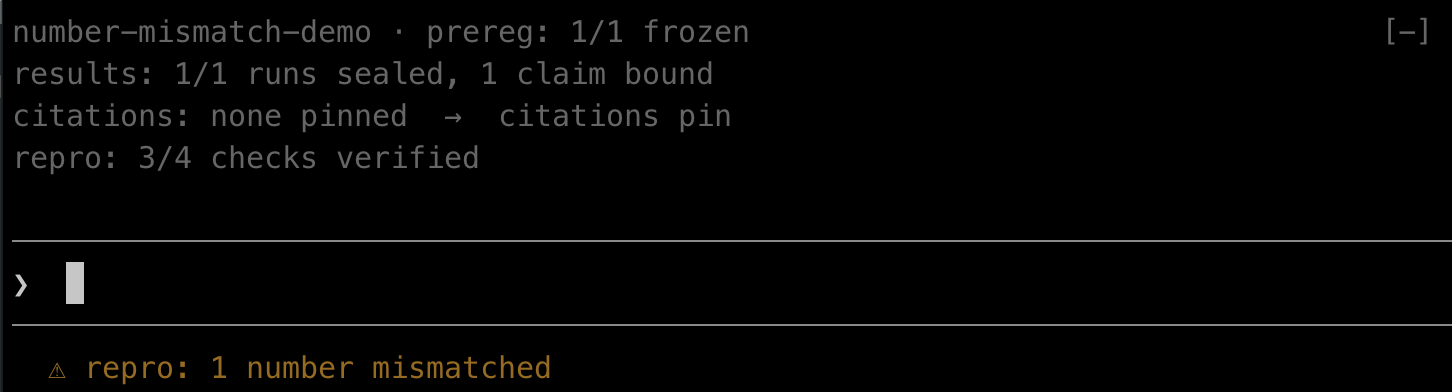
\includegraphics[width=0.92\textwidth]{figures/status_number_mismatch_2026-10-06b.png}
\caption{The state of a project's records as a session shows it. One plan is frozen, one run is
sealed with one claim bound to it, no quotation is pinned, and three of the manifest's four checks
verify. The line under the prompt reports the fourth: a number in the manuscript no longer matches
its results file.}
\label{fig:status}
\end{figure}

\section{Timing}
\label{sec:timing}

Each time in Section~\ref{sec:use} is the median of 10 runs of the command a user types, each in a
new process, on a 2019 16-inch MacBook Pro (\code{MacBookPro16,1}: 6-core Intel Core i7-9750H at
2.6\,GHz, 16\,GB of memory, macOS 26.5, Python 3.13.12), with version 0.5.2. \tVerifyCmd{} over
this paper's manifest ranges from 0.53 to 0.66 seconds, and \code{citations verify} over the
quotations this paper pins from 3.92 to 4.88 when every run reads every source. By default
\code{citations verify} keeps the text extracted from a source whose bytes have not changed, and
then takes 1.47 seconds.

Table~\ref{tab:timing} gives \tVerifyCmd{} over generated projects of increasing size, beside
\code{sha256sum -c} over the same artifacts, the least any check of pinned files can cost. Each
project holds a text, a table and a manifest of correspondence assertions, each tying a number in
the text to a cell of the table. The command starts in 0.192 seconds, which is most of its cost
up to 100 assertions. Artifact size adds what hashing adds: over 4\,GB the check takes 2.416
seconds and hashing alone takes 2.163. Time grows faster than the number of assertions past
10{,}000, because each text anchor is searched for across the whole text.

\begin{table}[H]
\centering
\small
\caption{Seconds to verify a generated project, by the number of assertions and by the bytes of
the artifacts they are checked against. Each time is the median of 5 runs, each in a new process,
of version 0.5.2 on a GitHub-hosted runner (\code{ubuntu-24.04}: AMD EPYC 9V45, 2 processors,
7\,GB of memory, Python 3.12.15). The last four rows hold the assertions at 100 and add pinned
files that no assertion reads.}
\label{tab:timing}
\begin{tabular}{@{}rrrr@{}}
\toprule
\textbf{Assertions} & \textbf{Artifact bytes} & \textbf{\tVerifyCmd{}} & \textbf{\code{sha256sum -c}} \\
\midrule
10 & 647 & 0.213 & 0.001 \\
100 & 6{,}389 & 0.238 & 0.001 \\
1{,}000 & 63{,}807 & 0.556 & 0.001 \\
10{,}000 & 638{,}009 & 6.733 & 0.002 \\
100{,}000 & 6{,}380{,}011 & 193.128 & 0.005 \\
\midrule
100 & 1{,}054{,}965 & 0.223 & 0.002 \\
100 & 16{,}783{,}605 & 0.246 & 0.010 \\
100 & 268{,}441{,}845 & 0.372 & 0.142 \\
100 & 4{,}294{,}973{,}685 & 2.416 & 2.163 \\
\bottomrule
\end{tabular}
\end{table}

% The toolkit over CODECHECK certificates. Drafted in the reproducible-science-codecheck
% repository (paper/appendix_certified_reproductions_v1c.tex). Every number is in
% artifacts/codecheck_indices.json, artifacts/codecheck_agreement_summary.json,
% artifacts/codecheck_mismatch_review.json or artifacts/codecheck_eligibility_summary.json.

\section{Certified reproductions}
\label{sec:codecheck}

CODECHECK issues a certificate when an independent codechecker regenerates a paper's outputs, and
each certificate's manifest names the regenerated files and the figure or table each belongs to
\citep{nust2021codecheck}. The correspondence between file and table
is therefore written by a third party. We run \tVerifyCmd{} over the public register to measure
how much of a certified reproduction can be checked number by number. The plan is registered
before any output file is opened.

\paragraph{Result.} Six certificates link fifteen tables to regenerated files, and 338 of the
713 numbers those tables print are bound to a cell of a file. In 326 of the 338, the paper and the
certificate's file hold the same number. Twelve differ, in two certificates, and each difference
has a cause that can be read from the files (Table~\ref{tab:cc-differences}). The counts describe
what can be checked in certified reproductions and do not estimate how often published numbers
are wrong.

\paragraph{From the register to checkable tables.} Table~\ref{tab:cc-funnel} follows the
register down to the certificates the toolkit can use. The manifests name 545 outputs, of which
419 are figures. Six certificates name a file the toolkit reads, keep it in their repository,
and say which table of the paper it holds.

\vspace{0.5em}
\begin{table}[H]
\centering
\small
\caption{Certificates in the CODECHECK register that reach each condition. Three certificates
describe their files without naming a table, and four name a file their repository does not
hold under that name.}
\label{tab:cc-funnel}
\begin{tabular}{@{}>{\raggedright\arraybackslash}p{0.74\textwidth}r@{}}
\toprule
condition & certificates \\
\midrule
in the register & 133 \\
names an output in a format read as values, not marked as outside the manuscript & 13 \\
that output is in the certificate's repository & 9 \\
its manifest comment names a table the paper has & 6 \\
\bottomrule
\end{tabular}
\end{table}

\paragraph{Coverage.} A number is bound when it has one address in the paper's extracted text
and one cell in the regenerated file. The bindings are written with Claude Code (Anthropic) from
views of each output in which every value is masked, and are locked before any comparison runs.
Four certificates bind between 64 of 92 and 137 of 140
numbers (Table~\ref{tab:cc-coverage}). Two bind none: their outputs hold formatted text, in one
a median with its interval and units in each cell and in the other a single column named
\code{text}. An output that reproduces a table's appearance has no cell to compare a number
against.

\vspace{0.5em}
\begin{table}[H]
\centering
\small
\caption{Numbers printed in linked tables, counting at most 60 per table, numbers bound on both
sides, and bound numbers that are the same in the paper and in the certificate's file.}
\label{tab:cc-coverage}
\begin{tabular}{@{}lrrrr@{}}
\toprule
certificate & printed & bound & same number & differ \\
\midrule
2025-018 & 140 & 137 & 133 & 4 \\
2020-025 & 90 & 86 & 86 & 0 \\
2022-001 & 92 & 64 & 56 & 8 \\
2024-020 & 58 & 51 & 51 & 0 \\
2020-011 & 33 & 0 & --- & --- \\
2020-008 & 300 & 0 & --- & --- \\
\midrule
all & 713 & 338 & 326 & 12 \\
\bottomrule
\end{tabular}
\end{table}

\paragraph{Agreement.} The toolkit reports 254 of the 338 bound numbers as agreeing at the
precision the paper prints. It reports 69 as disagreeing and does not read 15, and 72 of those
84 are the same number (Table~\ref{tab:cc-agreement}). The registered rule reads each output at the last commit before the certificate's check time.
Sixteen of 37 linked outputs exist there, so each output is read at the first commit holding
it, a change logged before any output is opened. The 30 numbers of one table of certificate
2020-025 differ from that first revision of its output file and equal the revision at the check
time in every cell; the certificate does not record which revision was certified. The 15 unread numbers, 11 of them equal to the file, expose a defect in the toolkit, whose
numeric parser rejects a thousands separator.

\vspace{0.5em}
\begin{table}[H]
\centering
\small
\caption{The 338 bound numbers, by how the paper's numeral compares with the certificate's
file.}
\label{tab:cc-agreement}
\begin{tabular}{@{}>{\raggedright\arraybackslash}p{0.66\textwidth}r@{}}
\toprule
comparison & numbers \\
\midrule
the toolkit reports agreement & 254 \\
the paper truncates where the toolkit rounds & 31 \\
equal at the output file's revision at the check time & 30 \\
equal once a thousands separator is removed & 11 \\
differ & 12 \\
\midrule
all & 338 \\
\bottomrule
\end{tabular}
\end{table}

\paragraph{Differences.} Table~\ref{tab:cc-differences} lists the 12 numbers that differ. Five
are standard deviations that equal the file's value multiplied by $\sqrt{(n-1)/n}$ with
$n = 1{,}070$, which is consistent with a paper that divides by $n$ where the regenerated file
divides by $n-1$; the same factor reproduces all 12 standard deviations counted in that table.
One regression coefficient is printed without its exponent. Three are memory measurements, 0.1\%
to 6.5\% from the file's value.

\vspace{0.5em}
\begin{table}[!ht]
\centering
\small
\caption{The 12 bound numbers that differ between the paper and the certificate's file. File
values are shortened to the digits needed to show the difference.}
\label{tab:cc-differences}
\begin{tabular}{@{}l>{\raggedright\arraybackslash}p{0.25\textwidth}rr>{\raggedright\arraybackslash}p{0.27\textwidth}@{}}
\toprule
certificate & quantity & paper & file & difference \\
\midrule
2022-001 & standard deviation & 30.33 & 30.3485 & divisor $n$ or $n-1$ \\
2022-001 & standard deviation & 21.80 & 21.8124 & divisor $n$ or $n-1$ \\
2022-001 & standard deviation & 28.20 & 28.2116 & divisor $n$ or $n-1$ \\
2022-001 & standard deviation & 84,154.56 & 84,193.92 & divisor $n$ or $n-1$ \\
2022-001 & standard deviation & 3,132.90 & 3,134.36 & divisor $n$ or $n-1$ \\
2022-001 & regression coefficient & 5.273 & $5.273 \times 10^{-7}$ & exponent not printed \\
2022-001 & median & 4,984.44 & 4,984.4349 & last printed digit \\
2022-001 & maximum & 827,067.40 & 827,067.43 & 0.03 \\
2025-018 & run time, seconds & 12.659 & 12.658475 & last printed digit \\
2025-018 & memory, megabytes & 3.1 & 2.897 & 6.5\% \\
2025-018 & memory, megabytes & 610.8 & 611.443 & 0.1\% \\
2025-018 & memory, megabytes & 2310.8 & 2329.968 & 0.8\% \\
\bottomrule
\end{tabular}
\end{table}

\paragraph{Planted changes.} Agreement means little if the toolkit cannot report a
disagreement, so each bound number is checked again on copies carrying one planted change
(Table~\ref{tab:cc-planted}). The toolkit reports a one-unit change in the last printed digit of
the file in all 254 cases and of the paper in 240. In ten of the fourteen misses the file stores
fewer digits than the paper prints, and in four the changed numeral sits among identical
neighbors that serve as its anchors. No deleted row, column or file is reported as agreement or
as a disagreement.

\vspace{0.5em}
\begin{table}[H]
\centering
\small
\caption{Planted changes on copies of the bound numbers, and how many the toolkit reports with
the outcome and reason its specification gives. The first three rows use the 254 numbers that
agree; the last three use all 338.}
\label{tab:cc-planted}
\begin{tabular}{@{}>{\raggedright\arraybackslash}p{0.44\textwidth}>{\raggedright\arraybackslash}p{0.30\textwidth}r@{}}
\toprule
planted change & expected report & as expected \\
\midrule
none & agreement & 254 of 254 \\
last printed digit of the file's value & disagreement & 254 of 254 \\
last printed digit of the paper's value & disagreement & 240 of 254 \\
addressed row deleted & row absent & 338 of 338 \\
addressed column deleted & column absent & 338 of 338 \\
output file deleted & not checked, file missing & 338 of 338 \\
\bottomrule
\end{tabular}
\end{table}


\section{Outside timestamps}
\label{sec:timestamps}

\code{prereg freeze} takes one SHA-256 digest over the plan and sends that digest, and nothing
else, to the OpenTimestamps calendar servers \citep{todd2016opentimestamps}. The proof they return
is kept beside the plan and committed with it. A proof is pending until the calendars commit it
into a Bitcoin block, whose date neither the author nor a calendar operator can change, usually
within hours; \code{prereg timestamp} then completes it and reports
the block and its date, the latest date at which the plan could have been written.
\code{prereg check} reads the proof without the network and fails when the proof is of a digest
other than the frozen one. No option skips the request: a freeze made with no network succeeds and
reports the timestamp as owed on every check until it is made. \code{results timestamp} dates the
head of the ledger the same way. The date is then held by a public record the author cannot
rewrite, which a repository's own history is not.

% Generated by scripts/build_audit_appendix.py from paper/audit/audits/*.yaml. Do not edit.
\section{Reproducible Science Audits}
\label{sec:catches}

This appendix audits 3 preregistered studies conducted with Reproducible Science:
two under journal review and one in progress. Each audit gives a
description of the study, an example finding, what each command found in its repository,
and the findings made while it was written. Table~\ref{tab:audits-clone} gives the result from
a clone for the two under review, and Table~\ref{tab:catches} their findings.

\begin{table}[!ht]
\centering
\small
\caption{What Reproducible Science established from a clone of each project, at the pinned commit.}
\label{tab:audits-clone}
\begin{tabular}{@{}>{\raggedright\arraybackslash}p{0.19\textwidth}c>{\raggedright\arraybackslash}p{0.25\textwidth}>{\raggedright\arraybackslash}p{0.17\textwidth}>{\raggedright\arraybackslash}p{0.16\textwidth}@{}}
\toprule
project & appendix & registered plans & quotations & ledger \\
\midrule
Cross-design evidence discordance & \ref{sec:audit-cross-design} & 4 of 6 registrations unchanged, 1 appended, 1 changed & 175 of 175 found & not in the repository \\
Knockout epistasis & \ref{sec:audit-knockout} & 3 of 3 plans unchanged & 18 declared, sources absent & chain intact, 153 events \\
\bottomrule
\end{tabular}
\end{table}

Findings are coded from each project's records: commits, ledger events, plan logs, claim files and
session transcripts. A finding counts
when a command, a script that performed the same check before the command existed, a hook, or an act
Reproducible Science requires (sealing an input, binding a number, pinning a
quotation) exposed it and a record says so. The coding rules were fixed before the records were read.
Defects found by a person or raised in review are not counted as findings.

\begin{table}[!ht]
\centering
\small
\setlength{\tabcolsep}{4pt}
\caption{Findings, by project and severity. A \emph{claim} finding would change a
reported number or conclusion. A \emph{source} finding is a value or reference attributed to a work
that does not contain it. A \emph{record} finding is a break in provenance that leaves every reported number
correct.}
\label{tab:catches}
\begin{tabular}{@{}lcrrrrr@{}}
\toprule
project & appendix & claim & source & record & cosmetic & total \\
\midrule
Cross-design evidence discordance & \ref{sec:audit-cross-design} & 5 & 14 & 8 & 4 & 31 \\
Knockout epistasis & \ref{sec:audit-knockout} & 3 & 2 & 10 & 3 & 18 \\
\midrule
total & & 8 & 16 & 18 & 7 & 49 \\
\bottomrule
\end{tabular}
\end{table}

\clearpage
\section{Audit: Cross-design evidence discordance}
\label{sec:audit-cross-design}

\paragraph{Description.} A preregistered study of drug-trial outcomes \citep{tower2026crossdesign}.\footnote{\url{https://github.com/elliottower/cross-design-evidence-discordance}, commit \code{c6a7a06}.}
The clone carries 365 tracked files, 6 registration documents, 94 claim records, 175 quotations and 75 bibliography entries.

\paragraph{All Findings.} 31: 5 claim, 14 source, 8 record, 4 cosmetic.

\paragraph{Example Finding.} \code{results verify} found two recorded files edited since they were recorded and one that had moved.

\paragraph{Reviews.} Of the 31 findings: 0 before submission, 11 review round 1, 2 review round 2, 0 review round 3, 17 review round 4, 1 after round 4.

\begin{table}[!ht]
\centering
\small
\caption{Cross-design evidence discordance: what each command found in a clone at the pinned commit, and what it could not establish. Exit 0 is a pass, 1 a finding, and 2 nothing to read.}
\label{tab:audit-cross-design-clone}
\begin{tabular}{@{}>{\raggedright\arraybackslash}p{0.13\textwidth}r>{\raggedright\arraybackslash}p{0.39\textwidth}>{\raggedright\arraybackslash}p{0.34\textwidth}@{}}
\toprule
command & exit & what it found & what it could not establish \\
\midrule
\code{prereg} & 1 & 6 registration documents, each frozen by a commit recorded in the document: 4 unchanged, 1 with text added after the frozen text, and 1 changed after its freeze & whether a registration was written before the outcomes it governs were seen \\
\code{results} & 2 & no ledger & which run any reported number came from \\
\code{citations} & 0 & 175 of 175 quotations found in their sources; 67 of the 94 sources were read from the library and matched to the SHA-256 the record pins & whether a quotation supports the sentence that cites it \\
\code{citations audit} & 0 & 75 bibliography entries, 74 carrying an identifier; 64 agree with the record the identifier resolves to and 10 disagree & whether the entry with no identifier is correct \\
\code{repro} & 2 & no evidence manifest & any assertion, none having been declared \\
\bottomrule
\end{tabular}
\end{table}

\begin{table}[!ht]
\centering
\small
\caption{Reviewer comments (4 reviewers, 6 reports) and findings for the cross-design study, by kind.}
\label{tab:audit-cross-design-review}
\begin{tabular}[t]{@{}lr@{}}
\toprule
Reviewer comments & Count \\
\midrule
design and argument & 20 \\
reporting and presentation & 12 \\
statistical method & 10 \\
references & 1 \\
code and data availability & 0 \\
other & 2 \\
\midrule
Total & 45 \\
\bottomrule
\end{tabular}
\hspace{3em}
\begin{tabular}[t]{@{}lr@{}}
\toprule
Findings & Count \\
\midrule
value or citation absent from the cited source & 9 \\
value differing from its source & 6 \\
wrong reference metadata & 11 \\
number bound to no run & 2 \\
other record findings & 3 \\
\midrule
Total & 31 \\
\bottomrule
\end{tabular}
\end{table}

\clearpage
\section{Audit: Knockout epistasis}
\label{sec:audit-knockout}

\paragraph{Description.} A study of knockout epistasis in Boolean gene regulatory networks, also covered in Section~\ref{sec:comparative} \citep{tower2026knockout}.\footnote{\url{https://github.com/elliottower/knockout-epistasis-dynamics}, commit \code{cb82384}.}
The clone carries 1{,}267 tracked files, 3 registered plans, 153 ledger events, 13 runs, 131 manuscript claims bound to a run, 7 claim records and 18 quotations.

\paragraph{All Findings.} 18: 3 claim, 2 source, 10 record, 3 cosmetic.

\paragraph{Example Finding.} Binding the manuscript's numbers to runs required recomputing them, and the recomputation revealed that a property stated for all 28 networks holds only for 27.

\begin{table}[!ht]
\centering
\small
\caption{Knockout epistasis: what each command found in a clone at the pinned commit, and what it could not establish. Exit 0 is a pass, 1 a finding, and 2 nothing to read.}
\label{tab:audit-knockout-clone}
\begin{tabular}{@{}>{\raggedright\arraybackslash}p{0.13\textwidth}r>{\raggedright\arraybackslash}p{0.39\textwidth}>{\raggedright\arraybackslash}p{0.34\textwidth}@{}}
\toprule
command & exit & what it found & what it could not establish \\
\midrule
\code{prereg} & 0 & 3 plans, each unchanged against the digest recorded when it was frozen & whether a plan was written before the outcomes it governs were seen \\
\code{results} & 1 & chain intact and anchored at 153 events; 8 of 12 recorded files match their digest and 4 carry more than one recorded digest & what share of the manuscript's numbers the 131 claims cover, the manuscript not being in the repository \\
\code{citations} & 1 & 18 quotations declared against 7 sources, each carrying a SHA-256; none checked, the sources not being in the repository & whether any quotation occurs in its source \\
\code{repro} & 2 & no evidence manifest & any assertion, none having been declared \\
\bottomrule
\end{tabular}
\end{table}


\clearpage
% The toolkit under a literature census run by a language model and coding agents: an audit block
% in the format of the generated audit pages, then how the toolkit is used during the study.
% Every count is read from paper/artifacts/census_counts.json, written by
% scripts/derive_census_counts.py from the audit record paper/audit/census_audit.json and from the
% study's repository at the commit that record pins, and bound in this paper's ledger to the run
% census-audit-2026-10-08.

\section{Audit: Literature census of 43{,}462 abstracts}
\label{sec:census}

\paragraph{Description.} A preregistered literature census of proteome-wide Mendelian randomization
papers, in progress.\footnote{Registration: \url{https://osf.io/zae8c}. The audit is of the study's repository at commit \code{62f181c}.}
It counts how often a protein--outcome claim is repeated, and how often the repeats rest on
overlapping data. The frozen plan is registered on OSF through \code{prereg register}, and the
plan's log records the registration and each amendment.
The repository carries 1 frozen plan with 194 log lines, 233
ledger events, 40 runs, 3{,}508 claim records and 23{,}939 quotations.

\paragraph{Example Finding.} \code{results verify --files} reports one sealed test file as recorded
with 2 different hashes: it was corrected in place and sealed again, against the study's rule that
a fix is a new file. No command clears the report.

\begin{table}[H]
\centering
\small
\caption{Literature census: what each command found in the repository, and what it could not establish. Exit 0 is a pass, 1 a finding, and 2 nothing to read.}
\label{tab:census-commands}
\begin{tabular}{@{}>{\raggedright\arraybackslash}p{0.13\textwidth}r>{\raggedright\arraybackslash}p{0.39\textwidth}>{\raggedright\arraybackslash}p{0.34\textwidth}@{}}
\toprule
command & exit & what it found & what it could not establish \\
\midrule
\code{prereg} & 0 & 1 plan, unchanged against the digest recorded when it was frozen & whether the plan answers the question \\
\code{results} & 1 & chain intact at 233 events; 373 of 374 recorded files match their digest and 1 carries 2 recorded digests & which run a reported number came from, no number being in a manuscript yet \\
\code{citations} & 1 & 13{,}989 of 13{,}989 pinned source sentences and 2{,}167 of 2{,}167 pinned sentences behind the dataset codes found in their stored sources; 7{,}783 quotations in the repository's own claims folder unchecked, their sources not being in the repository & whether a found sentence was read correctly \\
\code{repro} & 0 & 5 of 5 assertions verified & any count of the census, the assertions covering the search counts the plan states \\
\bottomrule
\end{tabular}
\end{table}

\subsection*{Application: Toolkit use during the study}

The census is conducted with the toolkit. A census of this size, run by a language model and by
coding agents in separate sessions, could not be audited or called confirmatory without the records
of Table~\ref{tab:census}. Each extraction can be checked against its source sentence, and each
rule is dated against what had been seen.

\begin{table}[H]
\centering
\small
\caption{The record kept at each stage of the census, and the command that keeps it. A review of
this kind ordinarily reports one count per stage.}
\label{tab:census}
\begin{tabular}{@{}>{\raggedright\arraybackslash}p{0.15\textwidth}>{\raggedright\arraybackslash}p{0.12\textwidth}>{\raggedright\arraybackslash}p{0.64\textwidth}@{}}
\toprule
\textbf{Stage} & \textbf{Command} & \textbf{Record} \\
\midrule
plan & \tPlan{} & one plan frozen before screening, and 194 dated log lines under it, each stating what had been seen when it was written \\
screening and extraction & \tRun{} & 90 seals of scripts and inputs and 40 recorded runs, over 43{,}462 abstracts screened and 14{,}053 claim records extracted \\
verification & \tCite{} & the source sentence of each of the 14{,}053 claim records, checked against the stored abstract \\
dataset coding & \tCite{} & 2{,}167 pinned sentences behind the codes for 872 dataset names \\
access to output & \tRun{} & 26 access records, each with what was shown and its level \\
\bottomrule
\end{tabular}
\end{table}

\paragraph{Model extraction.} A language model screens 43{,}462 abstracts and extracts 14{,}053
claim records from the 2{,}363 papers it admits. Each record carries the sentence it was drawn
from, so \code{citations verify} decides for every record whether the model quoted the abstract.
Of the 14{,}053 sentences, 13{,}989 resolve in the stored abstract. Of the 64 that do not, 27
occur twice in the abstract and 37 leave out one word of it. A found sentence establishes nothing
about whether the model read it correctly.

\paragraph{Agent coding.} Coding agents assign a dataset to each of 872 dataset names in 434
papers. An agent's code counts only when \code{citations pin} finds the sentence it rests on in the
source and that sentence holds an identifier unique to the coded release. Across four passes of
separate sessions, a script applies that rule to every code, and the coordinating agent asks each
session for counts and file paths and never for values.

\paragraph{Access to output.} Each access to output is a ledger record with a level. Of 26
accesses, 4 are at the level \emph{metadata only}, 19 at \emph{structure seen} and 3 at
\emph{outcomes seen}: a registered negative-control result, the text of three evidence
sentences printed by accident during a count, and the opening lines of one batch of the second
check, printed to learn its format. None shows a quantity either hypothesis concerns.
The plan was frozen before all three, so each confirmatory number is still recorded as confirmatory,
with the freeze it rests on named beside it.


\end{document}
